\chapter{Antecedentes}\label{chap:antecedentes}

\drop{E}s muy importante conocer un mínimo de información acerca de las áreas de trabajo que se pretenden abordar para la realización de un proyecto. Ya que el conocimiento es poder, y el hecho de leer sobre el trabajo que ha dedicado nuestra civilización previamente al nuestro, nos puede ayudar a evitar errores que en su día fueron quebraderos de cabeza para otros.

\begin{definitionlist}
\item[Sección \ref{sec:paradigmaVehiculos}: \nameref{sec:paradigmaVehiculos}]Complejidad y factores a tener en cuenta para el desarrollo de un vehículo autónomo.
\item[Sección \ref{sec:hardwareReconfigurable}: \nameref{sec:hardwareReconfigurable}] Ventajas y desventajas de la utilización de hardware reconfigurable.
\end{definitionlist}

\section{Coches autónomos}\label{sec:paradigmaVehiculos}

El hecho de que un sistema sea capaz de hacer llegar un vehículo de un lugar a otro sin poner en riesgo la integridad del entorno, y de sí mismo, es complejo. Ya que hay infinidad de sucesos que pueden ocurrir dando lugar a una colisión. Sin tener en cuenta otros sucesos como por ejemplo que el vehículo no llegue al destino correcto o tome una ruta  que sea más larga de lo que debería. Es por ello, que al ser tan extenso el número de posibilidades que afronta este sistema es necesario acotar el problema. Y aún así, el número de factores externos e internos que hay que tener en cuenta son muchos.

En esta sección se va a tratar de poner en situación al lector sobre la situación actual de los coches autónomos para comprender el porqué se ha decidido realizar este proyecto y de los factores que se deben tener en cuenta para el desarrollo de un coche autónomo que cumpla los objetivos de este \ac{TFG}.

\subsection{Situación actual de los coches autónomos}

Hoy en día las compañías automovilísticas están introduciendo funciones autónomas en sus coches. Un claro ejemplo son los coches que aparcan solos o que circulan de manera prácticamente autónoma por autovía. 

Hay que tener en cuenta que se pueden diferenciar distintos niveles de autonomía en un coche, ya que no tiene la misma complejidad conseguir que un vehículo aparque en bateria frente a lograr una conducción totalmente autónoma por ciudad. Es por esto que la \ac{SAE} \cite{SAE} decidío estandarizar la \emph{división en 6 niveles} \cite{SAEstandard} de la capacidad de conducción autónoma de un vehículo:

\begin{enumerate}
\item \textbf{Nivel 0}. El coche no tiene ningún sistema automatizado que le permita tomar el control, sólo puede tener sistemas que emitan alguna advertencia.
\item \textbf{Nivel 1}. En este nivel los coches incluyen sistemas como el \emph{control de crucero}\footnote{Sistema electrónico que permite fijar una velocidad de marcha que se mantiene sin necesidad de que el conductor mantenga pisado el acelerador. El sistema se desactiva cuando se pisa el freno. Con sólo pulsar el correspondiente botón se recupera automáticamente la velocidad previamente seleccionada. Los más modernos incorporan un radar en la parte delantera del coche, de forma que pueden controlar también de forma automática la distancia con el vehículo que circula delante.} o la tecnología para mantener el coche en el carril.
\item \textbf{Nivel 2}. Aquí el vehículo puede denominarse \emph{semiautónomo}. El conductor debe permanecer en alerta por si en algún momento tiene que tomar el control del coche ya que éste puede no responder adecuadamente y es obligatorio que el sistema se desactive cuando el conductor tome el control. Un ejemplo de coche semiautónomo es el \textit{Mercedes-Benz Clase E} \cite{Mercedes}. Está a la venta desde marzo de 2016 y destaca por el denominado \emph{Drive Pilot} que es capaz de evitar la salida de la calzada sin la necesidad de que existan líneas de carril. Nunca un coche fabricado en serie fue capaz de guiarse por una carretera sin la ayuda de las líneas de carril hasta que salió este \textit{Mercedes-Benz}.
\item \textbf{Nivel 3}. Los vehículos pueden circular de forma autónoma en entornos controlados como autopistas. En este nivel podría encontrarse el sistema \emph{Autopilot} de \textit{Tesla} en el \textit{Model S} \cite{Tesla}. Es un sistema que está desactivado por defecto en el coche y que debe ser conectado voluntariamente por el conductor. Realiza constantes comprobaciones para asegurarse de que el conductor permanece atento y con las manos en el volante avisando mediante alertas sonoras y luminosas si no detecta las manos en él.
\item \textbf{Nivel 4}. Los coches autónomos pueden circular sin supervisión del conductor en áreas acotadas donde el coche tenga suficiente información para no depender del conductor. Algunas empresas muy potentes ya han comenzado a hacer sus primeras pruebas serias para ver cuál es el funcionamiento real de los coches autónomos. \textit{Google} es un ejemplo de conducción autónoma; desde mayo de 2012 tiene licencia para probar coches autónomos en algunos estados de Estados Unidos. \textit{Volvo} y \textit{Uber} también se han aliado para crear la primera flota de taxis autónomos del mundo. Y otras marcas como \textit{BMW}, \textit{Citröen} o \textit{Audi} también se han lanzado a las pruebas con los coches autónomos.
\item \textbf{Nivel 5.} La conducción autónoma en este nivel es completa. Puede circular por cualquier carretera o ciudad siempre y cuando sea legal la conducción autónoma. Gracias a la tecnología, el coche podrá reaccionar ante cualquier imprevisto. Y no sólo los fabricantes de automoción están interesados en crear coches autónomos, otras empresas tecnológicas también indagan en el tema. Por ejemplo, \textit{Microsoft} está diseñando aplicaciones que puedan formar parte de estos vehículos \cite{Microsoft}. La marca china \textit{Baidu} ya prueba su coche \cite{Baidu}, mientras \textit{Apple} podría estar detrás de un proyecto de vehículo autónomo que, de momento, ofrece más rumores que realidades \cite{Apple}.
\end{enumerate}

Después de conocer acerca de los seis niveles de autonomía, este sistema que se pretende desarrollar en este \ac{TFG} emulará una autonomía de nivel 4. Esto es debido a que el sistema será capaz de analizar la información tomada y comunicará los movimientos pertinentes al vehículo de tal forma que no necesite la supervisión del ser humano. A continuación vamos a ver qué factores se deben tener en cuenta para el desarrollo de este \ac{TFG}.

\subsection{Factores a tener en cuenta para el desarrollo de un coche autónomo}

En primer lugar hay que entender que el sistema no va a resolver ninguna situación que no se haya implementado. Dicho de esta forma suena muy evidente pero hay situaciones que al comienzo del planteamiento del problema no se tienen en cuenta. Esto es debido a que el mero hecho de hacer funcionar el sistema en escenarios distintos puede provocar que en alguno de ellos no funcione como se esperaba. Debido a cuestiones como la luz, la composición del suelo, las características meteorológicas, el tamaño del escenario, etc... Por ello, es importante definir el tipo de escenario en el cual se va a desarrollar el proyecto para estudiar las diferentes características del entorno a las cuales se va a enfrentar el vehículo. Una vez definido el escenario sobre el cual se va a desarrollar el cálculo de la trayectoria del vehículo, hay que realizar pruebas con el dispositivo que deseamos utilizar para tomar la información del escenario. Existen diferentes formas de tomar la información pero en este \ac{TFG} se decidió utilizar una cámara desde el principio con el objetivo de que un futuro se utilizara hardware reconfigurable para optimizar el rendimiento. Por ello, se debe tener en cuenta que la información que obtenemos del entorno viene codificada en imágenes. Debido a que toda la información la tomamos de imágenes, debemos observar las diferentes situaciones que se pueden dar lugar en el entorno para tenerlas en cuenta en un futuro. Como por ejemplo, si la luz que existe en el escenario es constante o varía de una forma drástica dependiendo de la hora en la que se realicen las pruebas del sistema. 

Finalizadas las pruebas pertinentes con la cámara, se debe pensar si van a aparecer objetos en el escenario, ya que no es lo mismo calcular una trayectoria en un escenario sin objetos o con objetos que debe tener en cuenta a la hora de calcular la trayectoria para evitar colisionar con estos. Si existen objetos en el escenario en el cual se va a desarrollar el proyecto, se debe tener en cuenta que el dispositivo que toma la información del escenario debe detectar la posición de todos los objetos del entorno para evitar que la trayectoria pase por las coordenadas en las que se encuentren posicionados los objetos. Debido a esto nos surge la problemática acerca de cómo diferenciamos los objetos del entorno.

\subsubsection{Detección de objetos}

Para detectar objetos en una imagen, primero debemos plantearnos cómo diferenciar los objetos del entorno en el que se encuentran. Existen diferentes técnicas para distinguir los bordes\footnote{Se hace referencia a que los bordes son el perímetro de los objetos que hay en la imagen.} de la imagen:

\begin{figure}[hbtp]
 \centering
  \subfloat[Original]{
    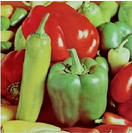
\includegraphics[width=0.25\textwidth]{./figures/Pimientos.jpeg}}
  \subfloat[Canny]{
    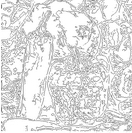
\includegraphics[width=0.25\textwidth]{./figures/PimientosCanny.jpeg}}
  \subfloat[Sobel]{
    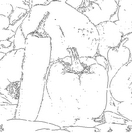
\includegraphics[width=0.25\textwidth]{./figures/PimientosSobel.jpeg}}
  \subfloat[Roberts]{
    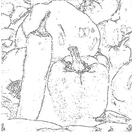
\includegraphics[width=0.25\textwidth]{./figures/PimientosRoberts.jpeg}}
 \caption{Ejemplo de funcionamiento de las técnicas enumeradas}
 \label{fig:AlgoritmosObjetos}
\end{figure}

\begin{enumerate}
\item Operador Roberts. Obtiene buena respuesta ante bordes diagonales. Ofrece buenas prestaciones en cuanto a localización. El gran inconveniente de este operador es su extremada sensibilidad al ruido\footnote{Se llama ruido a toda la información no deseada que se mezcla con la información útil que queremos procesar.} y por tanto tiene pobres cualidades de detección. \cite{OperadoresDeteccion} 
\item Operador Prewitt. En el operador Prewitt se involucran a los vecinos de filas o  columnas adyacentes para proporcionar mayor inmunidad al ruido. \cite{OperadoresDeteccion}
\item Operador Sobel. El operador Sobel, se supone que es más sensible a los bordes diagonales que el de Prewitt aunque en la práctica hay poca diferencia entre ellos. \cite{OperadoresDeteccion}
\item Algoritmo Canny. Es un algoritmo de múltiples fases para detectar un amplio rango de bordes. Es sin duda el operador más utilizado en la detección de bordes.\cite{Canny}
\end{enumerate}

Mediante la utilización de cualquiera de estas técnicas, figura \ref{fig:AlgoritmosObjetos}, se pueden detectar los bordes de los objetos, solo falta elegir en función de las características de nuestro escenario. Por ejemplo, si nuestra cámara percibe mucho ruido y elegimos la técnica del operador Roberts obtendremos muy malos resultados ya que el operador Roberts tiene una extrema sensibilidad al ruido y por lo tanto tiene pobres cualidades de detección.

\subsubsection{Delimitación de objetos}

Obtenidos los resultados de la detección de objetos, se puede apreciar el inconveniente de que el algoritmo de detección de bordes detecta el vehículo como un objeto. Esto es un problema, ya que para calcular la trayectoria que tomará el vehículo es necesario saber  el lugar en el que se encuentra, y dado que el vehículo debe ser autónomo se tiene que obtener la coordenada mediante el procesamiento de las imágenes tomadas por la cámara. Por ello, se debe pensar en alguna forma de diferenciar el vehículo del resto de objetos. Existen diferentes técnicas para diferenciar un objeto:

\begin{figure}
 \centering
  \subfloat[Detección de formas geométricas]{
  	\label{fig:FigurasGeometricas}
    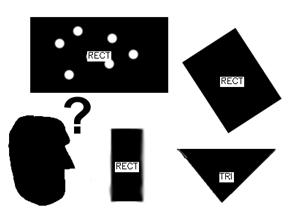
\includegraphics[width=0.4\textwidth]{./figures/FigurasGeometricas.jpeg}}
  \subfloat[Detección de objetos en función del color]{
  	\label{fig:AlgoritmoColor}
    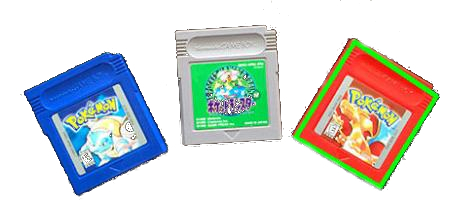
\includegraphics[width=0.6\textwidth]{./figures/AlgoritmoColor.jpg}}
 \caption{Ejemplos de algoritmos para la detección del vehículo}
 \label{fig:AlgoritmosVehiculo}
\end{figure}

\begin{enumerate}
\item Reconocimiento del vehículo debido a su forma geométrica. Existen algoritmos que sirven para detectar objetos según su forma geométrica. Figura \ref{fig:FigurasGeometricas}. Si al vehículo se le añade una forma geométrica característica, como por ejemplo un triángulo, el algoritmo será capaz de detectar en qué posición se encuentra esa forma geométrica, y por consiguiente el vehículo. \cite{FormasGeometricas}
\item  Establecer un patrón\footnote{Objeto, proceso o procedimiento que sirve para definir la unidad de una magnitud física.} al vehículo. Si el vehículo posee un tamaño característico que se diferencie de los demás objetos se puede diferenciar el vehículo detectando el tamaño exacto. Esta técnica tiene sus inconvenientes, ya que según dónde se encuentre la cámara el tamaño del objeto cambia. Y también se puede dar la casualidad de que aparezca un objeto en el entorno que tenga el mismo tamaño que el vehículo. Por ello se debe establecer un patrón al vehículo para poder reconocerlo. \cite{Patrones}
\item Existen algoritmos para la detección de objetos según su color. Por ejemplo, la librería \emph{OpenCV} \cite{OpenCV} contiene un algoritmo que consigue detectar un objeto en función de su color. \cite{AlgoritmoColor} Como se puede observar en la figura \ref{fig:AlgoritmoColor}. Pero existe el inconveniente de que aparezca en la imagen cualquier obstáculo que tenga el mismo color que el vehículo.
\end{enumerate}

Una vez se ha conseguido distinguir la posición en la que se encuentra el vehículo y la posición de los obstáculos que se encuentran en el entorno, se debe procesar esta información para realizar el cálculo de trayectoria que debe seguir el vehículo para evitar colisionar.

\subsubsection{Cálculo de trayectoria}

Existen diferentes tipos de algoritmos para calcular la trayectoria, es el diseñador el que debe elegir cuál de ellos se ajusta mejor al problema. Se van a describir una serie de algoritmos:

\begin{enumerate}
\item Algoritmo Djikstra \cite{AlgoritmoDjikstra}.  El algoritmo de dijkstra determina la ruta más corta desde un nodo\footnote{Es un punto de intersección, conexión o unión de varios elementos que confluyen en el mismo lugar} origen hacia los demás nodos, para ello es requerido como entrada un grafo\footnote{en el ámbito de las ciencias de la computación es un tipo abstracto de datos (TAD), que consiste en un conjunto de nodos (también llamados vértices) y un conjunto de arcos (aristas) que establecen relaciones entre los nodos} cuyas aristas posean pesos\footnote{El peso de un camino en un grafo es la suma de los pesos de todas las aristas atravesadas}. Si los pesos de las aristas son negativos no se puede usar el algoritmo de dijsktra, para pesos negativos tenemos otro algoritmo llamado Algoritmo de Bellmand-Ford \cite{AlgoritmoBellman}. Si los pesos de las aristas son de valor 1, entonces bastará con usar el algoritmo de \ac{BFS}.
\item Algoritmo \ac{BFS} \cite{AlgoritmoBFS}. Este algoritmo de grafos es muy útil en diversos problemas de programación. Por ejemplo, halla la ruta más corta cuando el peso entre todos los nodos es 1. Formalmente, \ac{BFS} es un algoritmo de búsqueda sin información, que expande y examina todos los nodos de un árbol sistemáticamente para buscar una solución. El algoritmo no usa ninguna estrategia heurística\footnote{Se conoce como heurística al conjunto de técnicas o métodos para resolver un problema. Para la informática, la heurística consiste en encontrar o construir algoritmos con buena velocidad para ser ejecutados.}.
\item Algoritmo A* \cite{AlgoritmoA}. El algoritmo A* es un algoritmo de búsqueda que puede ser empleado para el cálculo del camino más corto en una red. Se va a tratar de un algoritmo heurístico, ya que una de sus principales características es que hará uso de una función de evaluación heurística, mediante la cual etiquetará los diferentes nodos de la red y que servirá para determinar la probabilidad de dichos nodos de pertenecer al camino óptimo.
\end{enumerate}

Estos son algunos ejemplos de los algoritmos de cálculo de trayectoria existentes, pero si desea probar este tipo de algoritmos para poder obtener una visión más realista acerca de las ventajas y desventajas de cada algoritmo a simple vista, se recomienda acceder a la página web \cite{Algoritmos}, donde podrá definir usted mismo el entorno sobre el cual trabajará el algoritmo, así como decidir qué algoritmo utilizar, que heurística elegir y será posible ver la ejecución del algoritmo en directo.

Tras la elección del algoritmo de cálculo de trayectoria, es importante observar que el cálculo de la trayectoria en imágenes de gran resolución puede ser muy costoso en cuanto al tiempo de ejecución. Es decir, dado que el objetivo principal del proyecto es conseguir que un vehículo esquive en tiempo real los objetos que se encuentren en el entorno para llegar desde un punto de origen a un punto de destino. Se debe tener en cuenta el tiempo de ejecución de los algoritmos utilizados en el sistema. El algoritmo de cálculo de trayectoria forma el cuello de botella\footnote{En un proceso productivo, una fase de la cadena de producción más lenta que otras, que ralentiza el proceso de producción global.} del sistema debido a la cantidad de recursos que maneja. La resolución que utiliza la cámara  asignada al proyecto es \emph{full HD} (2.076.000 pixel por imagen). Es por ello que es muy importante la elección del algoritmo de cálculo de trayectoria ya que hay algunos que tardan más que otros.

\subsubsection{Comunicación}

Teniendo en cuenta que se ha conseguido un algoritmo que permite calcular la trayectoria en tiempo real, el siguiente paso que se debe plantear es cómo comunicar la solución al vehículo. Hay que tener en cuenta si los datos se van a transmitir por cable o de forma inalámbrica, ya que depende de la decisión que se tome el resultado puede verse afectado. Si por ejemplo se decide realizar la comunicación por cable, este puede llegar a limitar el movimiento del vehículo debido a que se enrede con algún obstáculo del entorno. Mientras que si se realiza de forma inalámbrica se debe tener en cuenta la distancia en la cual la transmisión de datos es segura. Es decir, si el vehículo se aleja demasiado la transmisión de datos puede verse afectada debido a la lejanía.

\subsubsection{Movimientos del vehículo}

Tomada la decisión acerca de qué tipo de comunicación se va a realizar, se debe tener en cuenta la forma en la que el vehículo debe traducir la información recibida en movimientos. Para ello se deben realizar una serie de pruebas acerca de cómo reacciona el vehículo a los estímulos recibidos. Estas pruebas son imprescindibles debido a que se desconoce cómo acelera el vehículo, qué respuesta de frenada tiene, así como la sensibilidad de giro que posee.

\section{Hardware reconfigurable}\label{sec:hardwareReconfigurable}

Una de las razones por las que se decidió tomar la información del sistema con la cámara es debido a que se tenía intención de embeber todo el sistema en hardware reconfigurable para optimizar el tiempo de ejecución y así poder lograr un funcionamiento del sistema en tiempo real. El hardware reconfigurable es aquél descrito mediante un lenguaje de descripción de hardware. Su naturaleza es completamente diferente a la del hardware estático\footnote{Es el conjunto de elementos materiales o tangibles de los sistemas electrónicos.}. Se desarrolla de una manera muy similar a como se hace con el software, mediante archivos de texto, que contienen el código fuente. Antes de profundizar acerca de cómo funciona el hardware reconfigurable se va a proceder a mostrar una serie de información acerca de \ac{FPGA}. 

Un \ac{FPGA} es un circuito integrado que, dicho en términos llanos, puede configurarse para llevar a cabo cualquier función lógica y hacer lo que a su dueño le plazca. Claro que para conseguir eso el diseñador debe programar/configurar el circuito, normalmente siguiendo la especificación de un lenguaje de descripción de hardware. Esto es algo así como preocuparse de implementar el código en el lenguaje \emph{C} o \emph{C++} sobre la funcionalidad del sistema, en vez de preocuparse en diseñar la electrónica digital del hardware. Una equiparación en forma de ejemplo sería si a la hora de conducir un vehículo sólo nos preocupamos de aprender las normas de circulación y cómo debemos manejar el vehículo para conducirlo, en vez de tener que diseñar y fabricar el vehículo previamente antes de poder aprender a conducirlo.

Por supuesto, en la práctica la creación está limitada por la capacidades de cada placa en la que se integra la \ac{FPGA}, así como de las limitaciones existentes acerca del uso de las herramientas de diseño. Como por ejemplo las funciones y librerías de programación a las que da soporte la herramienta.

A continuación se va a proceder a explicar qué tipo de herramientas son necesarias para la consecución del objetivo de este \ac{TFG}:

\begin{enumerate}
\item \emph{Vivado Design Suite} \cite{VivadoDS}. Con el uso de esta herramienta se genera el bitstream\footnote{Tecnología de transferencia de datos muy utilizada en gráfica y computación.} necesario para programar la placa \ac{FPGA}. Es decir, se incluyen e integran módulos con diferentes funciones para poder generar el sistema operativo sobre el que ejecutar el sistema que desarollemos. Llanamente hablando, se podría decir que con esta herramienta configuramos el hardware de tal forma que indicamos a la placa qué partes vamos a utilizar.
\item \emph{Vivado} \ac{SDK} \cite{VivadoSDK}. Esta herramienta nos permite programar y depurar el software que queremos incluir mediante un módulo en la placa. Como lenguajes de programación solo se pueden utilizar los lenguajes \emph{C} y \emph{C++} por lo que el entorno de desarrollo está enfocado a la programación en estos lenguajes. Este entorno tiene una funcionalidad muy parecida al \acx{IDE} \emph{Eclipse}. Un claro ejemplo de ello es la forma en la que se incluyen las librerías necesarias para el desarrollo del programa.
\item \emph{Vivado} \ac{HLS} \cite{VivadoHLS}. Mediante esta herramienta se puede realizar la simulación del funcionamiento del algoritmo en el lenguaje \emph{C} o \emph{C++}, la síntesis del algoritmo que se desea embeber en la placa \emph{Zedboard} partiendo de la descripción en \emph{C} o \emph{C++}, en vez de utilizar una descripción en \acx{VHDL}. La co-simulación que realiza una comparación con el modelo \acx{RTL} y finalmente el empaquetado del algoritmo para su programación en la placa. 
\item \emph{Petalinux} \cite{Petalinux}. Esta herramienta se ha utilizado para realizar la compilación de la aplicación del sistema para el procesador \ac{ARM} de la placa desde un ordenador con una distribución de x64 bits. Es decir, se ha realizado una compilación cruzada desde un ordenador con un procesador distinto emulando la configuración del procesador \ac{ARM}. Realizar la compilación del algoritmo en el procesador \ac{ARM} directamente es muy complejo ya que no tiene el mismo soporte que un procesador con distribución de x64 bits. Por ello, mediante el uso de esta herramienta se ha generado un directorio sobre el cual se emula la compilación en el procesador \ac{ARM} y así solo es necesario mover el fichero binario, generado en este directorio, a la placa para su ejecución.
\end{enumerate}
